\chapter {Preliminaries} \label{preliminaries}

This chapter discusses basic concepts from first-order logic that are used in the rest of this thesis. We will pay particular attention to their language and semantics since these are fundamental concepts necessary to understand the algorithmic constructions to compute interpolants. For a comprehensive treatment on the topic, the reader is suggested the following references \cite{10.5555/1642730, DBLP:books/daglib/0076838}.

\section{First-Order Predicate Logic}

\subsection{Language}
A language is a collection of symbols of different sorts equipped with a rule of composition that effectively tells us how to recognize elements that belong to the language \cite{DBLP:books/daglib/0080654}. In particular, a first-order language is a language that expresses boolean combinations of predicates using terms (constant symbols and function applications). In mathematical terms, 

\begin{definition}
 A first-order language (also denoted signature) is a triple $\langle \mathfrak{C}, \mathfrak{P}, \mathfrak{F} \rangle$ of non-logical symbols where:

\begin{itemize}
  \item $\mathfrak{C}$ is a collection of constant symbols
  \item $\mathfrak{P}$ is a collection of n-place predicate symbols
  \item $\mathfrak{F}$ is a collection of n-place function symbols
\end{itemize}

including logical symbols like quantifiers(universal ($\forall$), existential($\exists$)) logical symbols like parenthesis, propositional connectives (implication ($\rightarrow$), conjunction ($\land$), disjunction ($\lor$), negation ($\neg$)), and a countable number of variables \emph{Vars} (i.e. $\emph{Vars} = \{v_1, v_2, \dots\}$).

The rules of composition distinguish two objects, \emph{terms} and \emph{formulas}, which are defined recursively as follows:

\begin{itemize}
  \item Any variable symbol or constant symbol is a term.
  \item If $t_1, \dots, t_n$ are terms and $f$ is an n-ary function symbol, then $f(t_1, \dots, t_n)$ is also a term.
  \item If $t_1, \dots, t_n$ are terms and $P$ is an n-ary predicate symbol, then $P(t_1, \dots, t_n)$ is formula.
  \item If $x$ is a variable and $\psi, \varphi$ are formulas, 
    then $(\neg \psi), (\forall x . \psi), (\exists x . \psi)$ 
    and $(\psi \square \varphi)$ are formulas where $\square \in \{\rightarrow, \land, \lor\}$
  \item No other expression in the language can be considered terms nor formulas if such expressions are not obtained by the previous rules.
\end{itemize}

For notation purposes, we compactly represent a tuple $\langle x_1, \dots, x_n \rangle$ of variables as
$\cev{x}$. Abusing the notation, a formula of the form 
$\forall \cev{x} . \phi(\cev{x})$ (resp. $\exists \cev{x} . \phi(\cev{x})$)
denotes the formula $\forall x_1 . \forall x_2 \dots \forall x_n . \phi(x_1, \dots, x_n)$
(resp. $\exists x_1 . \exists x_2 \dots \exists x_n . \phi(x_1, \dots, x_n)$)

\end{definition}

\subsection{Semantics}

In order to define a notion of truth in a first-order language, it is necessary to 
associate for each non-logical symbol (since logical symbols have established 
semantics from propositional logic) a denotation or mathematical object and 
an \emph{assignment} to the collection of variables. The two previous 
components are part of a \emph{structure} \cite{DBLP:books/daglib/0076838} 
(or interpretation \cite{DBLP:books/daglib/0080654}) for a first-order language.

\begin{definition}
  Given a first-order language $\mathfrak{L}$, an interpretation $\mathfrak{I}$ is a pair $(\mathfrak{A}, \mathfrak{J})$, where $\mathfrak{A}$ is a non-empty domain (set of elements) and $\mathfrak{J}$ is a map that associates to the non-logical symbols from $\mathfrak{L}$ the following elements:
  \begin{itemize}
    \item $\mathfrak{I}$ assigns to each constant symbol $c$
      an elements $c^\mathfrak{A} \in \mathfrak{A}$
    \item $\mathfrak{I}$ assigns to each n-place
      predicate symbol $P$ an n-ary relation 
      $P^{\mathfrak{A}} \subseteq \mathfrak{A}^n$
    \item $\mathfrak{I}$ assigns to each n-place function
      symbol $f$ an n-ary operation $f^\mathfrak{A}$
      on $\mathfrak{A}$, i.e. $f^\mathfrak{A} : 
      \mathfrak{A}^n \rightarrow \mathfrak{A}$
  \end{itemize}

  An assignment $s : Vars \rightarrow \mathfrak{A}$ is a 
  map between variables to elements from the domain of 
  the interpretation.
\end{definition}

With the definition of interpretation $\mathfrak{I}$ and assignment $s$, we can recursively define a notion of \emph{satisfiability} (denoted by the symbol $\models_{\mathfrak{I}, s} $) as a free extension from atomic predicates (function application of predicates) to general formulas as described in \cite{DBLP:books/daglib/0076838}. For the latter, we need to extend the assignment function to all terms in the language.

\begin{definition}
  Let $\mathfrak{I} = (\mathfrak{A}, \mathfrak{J})$ be an interpretation and $s$ an assignment for a given language,
  Let $\bar{s} : Terms \rightarrow A$ be defined recursively as follows:
  \begin{itemize}
    \item $\bar{s}(c) = c^\mathfrak{J}$
    \item $\bar{s}(f(t_1, \dots, t_n)) = f^\mathfrak{J}(\bar{s}(t_1), \dots, \bar{s}(t_n))$
  \end{itemize}
\end{definition}

Notice that the extension of $s$ depends on the interpretation used.

\begin{definition}
  Given an interpretation $\mathfrak{I} = (\mathfrak{A}, \mathfrak{J})$, an assignment $s$, and $\psi$ a formula, we define $\mathfrak{I} \models_s \psi$ (read $\psi$ is satisfiable under interpretation $\mathfrak{I}$ and assignment $s$) recursively as follows:
  \begin{itemize}
    \item $\models_{\mathfrak{I}, s} P(t_1, \dots, t_n)$ 
      if and only if 
      $\langle
      \bar{s}(t_1), \dots, \bar{s}(t_n) \rangle 
      \in P^{\mathfrak{J}}$
    \item $\models_{\mathfrak{I}, s} \neg \psi$ if and only if  it is not the case that $\models_{\mathfrak{I}, s}   \psi$
    \item $\models_{\mathfrak{I}, s} \psi \land \varphi$ if and only if $\models_{\mathfrak{I}, s}  \psi$ and $   \models_{\mathfrak{I}, s}  \varphi$
    \item $   \models_{\mathfrak{I}, s}  \psi \lor \varphi$ if and only if $   \models_{\mathfrak{I}, s}  \psi$ or $   \models_{\mathfrak{I}, s}  \varphi$
    \item $   \models_{\mathfrak{I}, s}  \psi \rightarrow \varphi$ if and only if $   \models_{\mathfrak{I}, s}  \neg \psi$ or $   \models_{\mathfrak{I}, s}  \varphi$
    \item $   \models_{\mathfrak{I}, s}  \forall x . \psi$ if and only if for every $d \in \mathfrak{A},    \models_{\mathfrak{I}, s_{x \mapsto d}} \psi$, where $s_{x \mapsto d} : Vars \rightarrow \mathfrak{A}$ is reduct of $s$ under $Vars \setminus \{x\}$ and $s_{x \mapsto d}(x) = d$
    \item $   \models_{\mathfrak{I}, s}  \exists x . \psi$ if and only if exits $d \in \mathfrak{A},    \models_{\mathfrak{I}, s_{x \mapsto d}} \psi$, where $s_{x \mapsto d}$ is defined as in the previous item.
  \end{itemize}

  If an interpretation and assignment satisfies a formula, then we 
  say that the interpretation and the assignment are a model for the 
  respective formula. A collection of formulas is satisfied by 
  an interpretation and assignment if these model each formula 
  in the collection.

  A formula $\psi$ is said to be a \emph{valid} 
  formula of the interpretation $\mathfrak{I}$ 
  when $\models_{\mathfrak{I}, s} \psi$ for all 
  possible assignments $s$.

  Additionally, if all the models $(\mathfrak{I},
  s)$ in a language of a collection of formulas 
  $\Gamma$ satisfy a formula $\psi$, then we say 
  that $\Gamma$ logically implies $\psi$ 
  (written $\Gamma \models \psi$). For the 
  latter, $\psi$ is said to be a \emph{valid} 
  formula of the model $(\mathfrak{I}, s)$.

\end{definition}

%%% Local Variables:
%%% mode: latex
%%% TeX-master: "main"
%%% End:

\section{Mathematical Theories} \label{math_theories}

A theory $\mathcal{T}$ is a collection of formulas that are closed under logical implication, i.e. if $\mathcal{T} \models \psi$ then $\psi \in \mathcal{T}$. This concept is quite relevant for our thesis work since we will focus on two theories, the quantifier-free fragment of the theory of equality with uninterpreted functions (EUF), and the theory of unit two variable per inequality (UTVPI). 

For some theories it is enough to provide a collection of formulas (known as the axioms of the theory). For the case of the theories of interest for the thesis, the axiomatization if the following:

\subsection{Equality with uninterpreted functions}

\begin{definition} \label{euf_axioms}
  Let $\mathfrak{L}_{EUF} = \{ \{\}, \{ = \}, \{ f_1, \dots, f_n \} \}$ be the language of EUF. The axioms of the theory are:
  \begin{itemize}
    \item (Reflexivity) $\forall x . x = x$
    \item (Symmetry) $\forall x . \forall y . x = y \rightarrow y = x$
    \item (Transitivity) $\forall x . \forall y . \forall z. (x = y \land y = z) \rightarrow x = z$
    \item (Congruence) $\forall x_1  \dots \forall x_n . \forall y_1 \dots \forall y_n . (x_1 = y_1 \land \dots \land x_n = y_n) \rightarrow f(x_1, \dots, x_n) = f(y_1, \dots, y_n) $
  \end{itemize}
\end{definition}

We notice that the congruence axiom is not a first-order logic axiom, but rather an axiom-scheme since it is necessary to \emph{instantiate} such axiom for every arity of the function symbols in a given language.

\subsection{Ordered commutative rings}

In order to describe the UTVPI theory we will first introduce the language and theory of an ordered commutative ring.

\begin{definition}
  Let $\mathfrak{L}_{Ord-R} = \{, \{0, 1 \}, \{ = , \leq \}, \{+, -, * \}, \}$ be the 
  language of an ordered commutative ring $R$. The axioms of the theory are:
  \begin{itemize}
    \item $\forall x . \forall y . \forall z . x + (y + z) = (x + y) + z$
    \item $\forall x . \forall y .  x + y = y + x$
    \item $\forall x . x + 0 = x$
    \item $\forall x . x + (- x) = 0$
    \item $\forall x . \forall y . \forall z. x * (y * z) = (x * y) * z$
    \item $\forall x . x * 1 = x$
    \item $\forall x . \forall y .  x * y = y * x$
    \item $\forall x . \forall y . \forall z . x * (y + z) = x * y + x * z$
    \item $\forall x . \forall y . \forall z . (y + z) * x = y*x + z * x$
    \item $\forall x . \forall y . \forall z . x \leq y \rightarrow x + z \leq y + z$
    \item $\forall x . \forall y . (0 \leq x \land 0 \leq y) \rightarrow 0 \leq x * y$.
    \item $0 \neq 1 \land 0 \leq 1$ 
  \end{itemize}
\end{definition}

Section \ref{decision_procedures} discusses computability 
aspects for the theories of interest that are relevant 
for verification.

%%% Local Variables:
%%% mode: latex
%%% TeX-master: "main"
%%% End:

\section{Interpolants}

Following the notation in \cite{10.1007/11532231_26}, we denote 
$\mathcal{V}(\psi)$ to be the set of non-logical symbols, variables
and constants of formula $\psi$. Given an instance for the interpolation
problem $(A, B)$ \footnote{For the rest of the thesis, we will denote the 
  first formula of an interpolation problem as the A-part 
and the second component as the B-part}, 
we distinguish the following categories:

\begin{itemize}
  \item $\psi$ is \emph{A-local} if $\mathcal{V}(\psi) \in 
    \mathcal{V}(A) \setminus \mathcal{V}(B)$
  \item $\psi$ is \emph{B-local} if $\mathcal{V}(\psi) \in 
    \mathcal{V}(B) \setminus \mathcal{V}(A)$
  \item $\psi$ is \emph{AB-common} if $\mathcal{V}(\psi) \in
    \mathcal{V}(A) \cap \mathcal{V}(B)$
  \item $\psi$ is \emph{AB-pure} when either $\mathcal{V}(\psi) \subseteq 
    \mathcal{V}(A)$ or $\mathcal{V}(\psi) \subseteq \mathcal{V}(B)$, otherwise
    $\psi$ is \emph{AB-mixed}
\end{itemize}

\begin{example} \label{first_example}

  Consider the following interpolation pair: $(f(a + 2) + 1 = c + 1
    \land f(a + 2) = 0
  , f(c) \leq b \land b < f(0))$. With respect to the previous 
  interpolation pair, we can tell that:
  \begin{itemize}
    \item The formula $f(a + 2) = c$ is 
      AB-pure but not A-local nor B-local nor AB-common
    \item The formula $\neg(a \leq f(f(b) + 1))$ is an AB-mixed
      literal
    \item The formula $a + 1 = 1$ is A-local.
    \item The formula $c + 1 = 1$ is AB-pure but not AB-common.
    \item The formula $c = 0$ is AB-common.
    \item In general, $AB-common$ formulas are not $AB-pure$ formulas.
  \end{itemize}
\end{example}

\subsection{Craig interpolation theorem}

Let $\alpha, \beta, \gamma$ be logical formulas in a given theory. If
$\models_{\mathcal{T}} \alpha \rightarrow \beta$, we say that $\gamma$ is an
interpolant for the interpolation pair $(\alpha, \beta)$ if the following conditions
are met:

\begin{itemize}
\item $\models_{\mathcal{T}} \alpha \rightarrow \gamma$
\item $\models_{\mathcal{T}} \gamma \rightarrow \beta$
\item Every non-logical symbol in $\gamma$ occurs both in $\alpha$ and
  $\beta$.
\end{itemize}

The \emph{interpolation problem} can be stated naturally as 
follows: given two logical formulas $\alpha, \beta$ such that 
$\models_{\mathcal{T}} \alpha \rightarrow \beta$, find
the interpolant for the pair $(\alpha, \beta)$.

In his celebrated result \cite{10.2307/2963594}, Craig proved that for every pair
$(\alpha, \beta)$ of formulas in first-order logic such that
$\models \alpha \rightarrow \beta$, an interpolation formula exists. Nonetheless,
there are many logics and theories that this result does not hold \cite{komori1978}.

Usually, we see the interpolation problem defined differently in the literature, 
where it is considered $\beta^{'}$ to be $\neg \beta$ and 
the problem requires that the pair $(\alpha, \beta^{'})$
is mutually contradictory (unsatisfiable). This definition was popularized by 
McMillan \cite{10.1007/978-3-540-24730-2_2}. This shift of attention explains 
partially the further development in interpolation generation algorithms 
since many of these relied on SMT solvers that provided refutation proofs 
in order to (re)construct interpolants for different theories (and their 
combination) \cite{10.1007/978-3-642-02959-2_17, 
10.1007/978-3-642-36742-7_9, mcmillan2011interpolants}.

Relaxed definitions are considered to the interpolation 
problem when dealing with specific
theories \cite{10.1007/11532231_26} in a way that interpreted 
function can be also part of the interpolant. The latter is 
justified since otherwise, many interpolation formulas might not exist
in different theories or the interpolants obtained might not 
be relevant (for example, lisp programs). This is formalized as follows:

\begin{definition} \cite{10.1007/11532231_26}
  Let $\mathcal{T}$ be a first-order theory of a signature $\Sigma$ and 
  let $\mathcal{L}$ be the class of quantifier-free $\Sigma$ formulas.
  Let $\Sigma_\mathcal{T} \subseteq \Sigma$ denote a designated set
  of interpreted symbols in $\mathcal{T}$. Let $A, B$ be formulas
  in $\mathcal{L}$ such that $A \land B \models_{\mathcal{T}} \bot$.
  A \emph{theory-specific} interpolant for $(A, B)$ in $\mathcal{T}$
  is a formula $I$ in $\mathcal{L}$ such that 
  $A \models_{\mathcal{T}} I$, $B \land I \models_{\mathcal{T}} \bot$,
  and $I$ refers only to AB-common symbols and symbols in 
  $\Sigma_{\mathcal{T}}$.
\end{definition}

\begin{example}
  In example \ref{first_example} we can tell $c + 1 = 1$ is not an
  interpolant simplify because the symbol $1$ only appears on the
  A-part. However, if $\Sigma_{\mathcal{LIA(\mathbb{Z})}}$ contains the
  interpreted symbols of $LIA(\mathbb{Z})$ (i.e. $+, *, 0, 1, 2, \dots$),
  then $c + 1 = 1$ becomes a \emph{theory-specific} interpolant. 

  Notice that $c = 0$ is an interpolant even if the set of interpreted symbols 
  used for interpolation is empty.
\end{example}

\subsection{Uniform Interpolant}

A uniform interpolant is a particular kind of interpolant for an inconsistent
pair of formulas. Introduced in \cite{pitts1992} as a 
construction to provide an interpretation
for second order intuitionistic propositional logic 
\emph{$IpC^2$}
\footnote{I.e. $IpC^2$ quantifies over 
propositional variables.}
using intuitionistic propositional logic \emph{IpC}.
Our notion of uniform interpolant is taken 
from \cite{ghilardi2020compactly}
where the authors provide the following definition:

\begin{definition}
  Fix a theory $T$ and an existential formula $\exists \cev{e} . \phi(\cev{e}, \cev{z})$; call \emph{residue} of $\exists \cev{e} . \phi(\cev{e}, \cev{z})$ the following set of
  quantifier-free formulae:

  \begin{equation*}
    Res(\exists \cev{e} . \phi(\cev{e}, \cev{z})) = \{ \theta(\cev{z}, \cev{y}) | T \models \exists \cev{e} . \phi(\cev{e}, \cev{z}) \rightarrow \theta(\cev{z}, \cev{y}) \} =\{ \theta(\cev{z}, \cev{y}) | T \models \phi(\cev{e}, \cev{z}) \rightarrow \theta(\cev{z}, \cev{y}) \}
  \end{equation*}

  A quantifier-free formula $\psi(\cev{y})$ is said to be a \emph{T-uniform interpolant} 
  of $\exists \cev{e} . \phi(\cev{e}, \cev{z})$ if and only if $\psi(\cev{y}) \in Res(\exists \cev{e} \phi(\cev{e}, \cev{y}))$ and 
  $\psi(\cev{z})$ implies (modulo T)
  all the other formulae in $Res(\exists \cev{e} \phi(\cev{e}, \cev{y}))$.

  A theory $T$ has the \emph{Uniform Interpolation Property} 
  if every existential formula
  $\exists \cev{e} . \phi(\cev{e},\cev{y})$ has a T-uniform interpolant. 

\end{definition}

%%% Local Variables:
%%% mode: latex
%%% TeX-master: "main"
%%% End:

\section{Decision Procedures} \label{decision_procedures}

Given a theory $\mathcal{T}$ and a formula $\psi$ in 
the language of $\mathcal{T}$, is it possible to know 
$\models_{\mathcal{T}} \psi$? The last question is 
known as the decision problem for 
$\mathcal{T}$. This question has 
been studied extensively for many theories of interest 
\cite{borger2001classical}. 

Regarding the decidability of the theories 
discussed in the thesis work, it is known that 
the quantified EUF theory is undecidable \cite{borger2001classical}
Nonetheless, the quantifier-free fragment of EUF and 
the restriction imposed in the decision problem for 
the UTVPI theory allow efficient algorithms to decide 
validity and satisfiability in their respective theories 
\cite{10.1145/322186.322198, 10.1145/322217.322228, 
10.1007/11559306_9}. The ordered abelian group theory
is decidable as well \cite{DBLP:books/daglib/0076838}.

In the rest of this section we review some decision 
problems and provide references to their respective
decision procedures used in the implementation work of 
the thesis.

\subsection{Satisfiability and Satisfiability Modulo Theories}

The satisfiability problem consists of finding a 
propositional assignment for a propositional formula. 
This problem is at the core level of complexity theory, 
defining an important class of problems known as 
NP, which includes problems whose
algorithms seem to be intractable.
Developments in algorithms and heuristics 
\cite{10.5555/2898950, 
935565} have made it possible to use satisfiability 
algorithms 
to solve real-world problems in 
verification \footnote{These
  advances do not provide an answer to the well-known P vs. NP
  problem. There are results indicating a class of problem instances
  for many of the SAT algorithms which cannot be solved in less that
  \bigO{2^n} steps \cite{10.5555/2898950}.
}.

The DPLL algorithm \cite{10.1145/368273.368557} 
(and other extensions) is the algorithm
found in many SAT solvers. Fundamentally, it is a search-based algorithm
which implements operators (decide, unit-propagation, backtrack)
to find a satisfiable assignment. If the algorithm is not able to
find a satisfying assignment for a formula, then it is possible to 
extract a \emph{resolution proof} based on the traces of the search
operations.

\begin{example}

  \begin{figure}

    \centering

    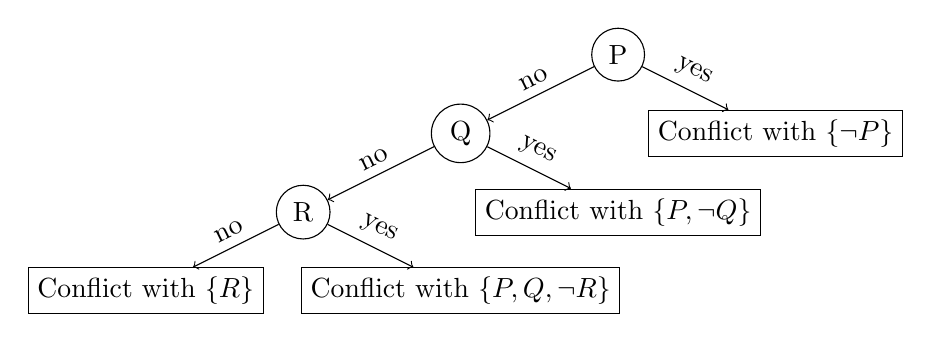
\begin{tikzpicture}[->]
      \node(p) at (6, 5) [circle, draw] {P};
      \node(q) at (4,4) [circle, draw] {Q};
      \node(r) at (2, 3) [circle, draw] {R};
      \node(expl1) at (8, 4) [rectangle, draw] {Conflict with $\{\neg P\}$};
      \node(expl2) at (6, 3) [rectangle, draw] {Conflict with $\{P, \neg Q\}$};
      \node(expl3) at (4, 2) [rectangle, draw] {Conflict with $\{P, Q, \neg R\}$};
      \node(expl4) at (0, 2) [rectangle, draw] {Conflict with $\{R\}$};

      \path[every node/.style={sloped,anchor=south,auto=false}]
      (p) edge node {yes} (expl1)   
      (p) edge node {no}  (q)   
      (q) edge node {yes} (expl2)
      (q) edge node {no}  (r)
      (r) edge node {yes} (expl3)
      (r) edge node {no}  (expl4);
    \end{tikzpicture}

    \caption{Example of DPLL execution on 
      $\{\{\neg P\}, \{P, Q, \neg R\}, \{R\}, 
    \{P, \neg Q\} \}$} \label{dpll_figure}

  \end{figure}

  We can see that the following resolution proof resembles the
  structure of the DPLL execution on figure \ref{dpll_figure}, i.e.
  if we rotate the proof-tree and mark the nodes by the pivots used
  we obtained a similar tree obtained by the execution of the DPLL
  algorithm. This fact becomes relevant because it enables us 
  to construct a resolution proof from the traces of a SAT 
  solver used
  in the theory combination part of the implementation. 

  \begin{figure}
    \centering
    \begin{prooftree}
      \hypo[]{\neg P}
      \hypo[]{P \lor Q \lor \neg R}
      \infer2[$res_P$]{Q \lor \neg R}
      \hypo[]{R}
      \infer2[$res_R$]{Q}
      \hypo[]{P \lor \neg Q}
      \infer2[$res_Q$]{P}
      \hypo[]{\neg P}
      \infer2[$res_P$]{\bot}
    \end{prooftree}
    \caption{Example of resolution proof} 
    \label{example_resolution_proof}
  \end{figure}

\end{example}

We can extend this approach to work not only with propositional
variables but with terms of more complex signatures 
\cite{10.5555/1391237}. If we are given a boolean combination 
of formulas from any theory that is capable of deciding the 
satisfiability of any conjunction of formulas in the theory, 
by using a \emph{lazy framework} integration with a SAT solver it is 
possible to find either a model or declare unsatisfiable such boolean
combination as follows: (i) first abstract the literals in the boolean
combination to (pseudo) boolean propositions; (ii) find a satisfying
assignment (using a SAT solver) of the (pseudo) boolean propositions;
(iii) using the theory solver, test if the collection of positive
and negative literals induced by the pseudo boolean variables is
satisfiable; (iv) if it is then declare the formula satisfiable, 
otherwise \emph{learn} (or block) the pseudo boolean clause obtained
(by negating the conjunction of boolean constraints) in the SAT
solver and repeat from step (ii); (v) if it is not possible to
find a satisfying assignment for the pseudo boolean variables, 
declare the original formula to be unsatisfiable.

These algorithms are used in the last section of the thesis work.
The implementation for the interpolation combination method
in \cite{10.1007/11532231_26} requires a resolution-based
proof in order to compute partial interpolants by integrating
Pudlak's algorithm.

%%% Local Variables:
%%% mode: latex
%%% TeX-master: "main"
%%% End:

\subsection{Congruence Closure}

The congruence closure problem consists of given a conjunction of
equalities and disequalities $\psi$ determine if an equality
$u = v$ follows from the consequence generated by $\models_{EUF} 
\psi$.

In \cite{10.1007/978-3-540-32033-3_33}, the authors 
introduced a Union-Find data structure that supports the 
Explanation operation. This operation receives as input 
an equation between constants. If the input equation is 
a consequence of the current equivalence relation defined 
in the Union Find data structure, the Explanation operation 
returns the minimal sequence of equations used to build 
such equivalence relation, otherwise it returns 
`Not provable'. A proper implementation of this algorithm 
extends the traditional Union-Find data structure with 
a \emph{proof-forest}, which consists of an additional 
representation of the underlying equivalence relation that 
does not compress paths whenever a call to the Find 
operation is made. For efficient reasons, the Find 
operation uses the path compression and weighted union.

The main observation in \cite{10.1007/978-3-540-32033-3_33} 
is that, in order to recover an explanation between 
two terms, by traversing the path between the two nodes 
in the proof tree, the last edge in the path guarantees to 
be part of the explanation. Intuitively, this follows because only 
the last Union operation was responsible of merging the 
two classes into one. Hence, we can recursively recover 
the rest of the explanation by recursively traversing 
the subpaths found.

Additionally, the authors in \cite{10.1007/978-3-540-32033-3_33} 
extended the Congruence Closure algorithm 
\cite{10.1007/978-3-540-39813-4_5} using the above data 
structure to provide Explanations for the theory of EUF. The congruence 
closure algorithm is a simplification of the congruence 
closure algorithm in \cite{10.1145/322217.322228}. The latter 
combines the traditional \emph{pending} and \emph{combine} list 
into one single list, hence removing the initial 
\emph{combination} loop in the algorithm in 
\cite{10.1145/322217.322228}.

%%% Local Variables:
%%% mode: latex
%%% TeX-master: "main"
%%% End:

\subsection{Satisfiability of Horn clauses of propositions and grounded equations}

TODO.

\subsubsection{Decision Problem}

TODO.

\subsubsection{Decision Procedure}

In \cite{GALLIER1987233} it was proposed an algorithm 
for testing the unsatisfiability
of ground Horn clauses with equality. The main idea was 
to interleave two algorithms: \emph{implicational propagation}
(propositional satisfiability of Horn clauses) that 
updates the truth value of equations in the antecedent 
of the input Horn clauses \cite{DOWLING1984267}; and 
\emph{equational propagation} (congruence closure for 
grounded equations) to update the state of a 
Union-Find data structure \cite{10.1145/364099.364331}
that keeps the minimal equivalence relation defined 
by grounded equations in the input Horn clauses.

The author in \cite{GALLIER1987233} defined two 
variations of his algorithms by adapting
the Congruence Closure algorithms in 
\cite{10.1145/322217.322228, 10.1145/322186.322198}.
Additionally, modifications in the data structures 
used by the original algorithms were needed
to make the interleaving mechanism more efficient.

TODO.

%%% Local Variables:
%%% mode: latex
%%% TeX-master: "main"
%%% End:

\subsection{Nelson-Oppen framework for theory and interpolation
combination}

The theory combination problem consists on taking a 
formula from the union of two (or more) disjoint 
languages and tell if such formula is satisfiable
or not in the combined theory, i.e. a theory resulting
after putting together two (or more) axiomatizations.

In \cite{10.1145/357073.357079} the authors defined a procedure
to achieve the above problem. The key idea is to \emph{purify} 
the sub-formulas by including additional constant 
symbols equating sub-terms such that the resulting formula 
can be splitted into components of the appropriate language 
for each theory solvers to work with. The separation naturally
will hide relevant information to the solvers, and they 
might not be able to decide satisfiability correctly.
The authors noticed that to solve the above problem it is enough to 
share disjunction of equalities between the combined theories of shared
terms. In addition, they proved that some theories have the 
following property:

\begin{definition}
  Let $\mathcal{T}$ be a theory. We say that $\mathcal{T}$
  is a \emph{convex theory} if a finite conjunction of formulas 
  in $\mathcal{T}$ $\psi = \bigwedge_{i = 1}^m \psi_i$ satisfies
  $\psi \models_{\mathcal{T}} \bigvee_{j = 1}^n 
  x_j = y_j$, then exists $k \in \{1, \dots, n \}$ such that 
  $\psi \models_{\mathcal{T}} x_k = y_k$.
\end{definition}

Hence, it is important to detect
whether the theories involved are convex or not since 
this can improve performance since convex theories do not
need to share disjunctions of equalities as mentioned before
(since all these disjunctions imply a single equality).

\begin{example}
  \begin{itemize}
    \item The conjunctive fragment of equality logic is an example
      of a convex theory since
      it can always decide the membership of an equation in the 
      equivalence relation. 
    \item The theory of UTVPI over the integers is an example of 
      non-convex theory. To see the latter consider
      $1 \leq x \land x \leq 2 \models_{UTVPI(\mathbb{Z})} 1 = x \lor 2 = x$.
      However, it is not the case that 
      $1 \leq x \land x \leq 2 \models_{UTVPI(\mathbb{Z})} 1 = x$
      nor 
      $1 \leq x \land x \leq 2 \models_{UTVPI(\mathbb{Z})} 2 = x$.
  \end{itemize}
\end{example}

An interpolation combination framework as proposed in \cite{10.1007/11532231_26}
follow the same idea towards theory combination. Inductively, they define
\emph{partial interpolants} for each shared equality/disjunction of equalities
until some theory reaches the unsatisfiable state, which is expected since 
an interpolant is a pair a mutually contradicting formulas.

This framework was implemented in the thesis work. This framework was chosen
in particular since it allows working with non-convex theories (in our case
for the theory of UTVPI over $\mathbb{Z}$).

%%% Local Variables:
%%% mode: latex
%%% TeX-master: "main"
%%% End:


%%% Local Variables:
%%% mode: latex
%%% TeX-master: "main"
%%% End:

\section{General system description}

TODO.

\subsection{Minor modifications to Z3}

TODO.

\subsection{Minor modifications to zChaff}

TODO.

%%% Local Variables:
%%% mode: latex
%%% TeX-master: "main"
%%% End:


%%% Local Variables:
%%% mode: latex
%%% TeX-master: "main"
%%% End:
